\documentclass{Beautybook-V6.1}
\coverstyle={
    cover-choose=en, % cn (需新增项\entitle{#}); en ; enfig ; birkar
}
\usepackage{rotating}
\tikzset{>=Stealth}
\setlist{nosep,font=\upshape} % 取消所有列表默认距离
% 浮动环境设置
% 默认情况下, \LaTeX{} 要求每页的文字至少占据 20%,否则该页就只单独放置一个浮动环境,
% 而这通常不是我们想要的, 我们将这个要求降低到 5%.
\renewcommand*{\textfraction}{0.05}
% 有时如果多个浮动环境连续放在一起,
% 会将它们分在几个不同页,即使它们可在同一页放
% 得下. 我们可以通过修改 |\topfraction| 和 |\bottomfraction| 分别设置顶端和底端的浮
% 动环境的最大比例.
\renewcommand*{\topfraction}{0.9}
\renewcommand*{\bottomfraction}{0.8}
% 有时\LaTeX{}会把一个浮动环境单独放在一页,
% 我们要求这个环境至少要占据 85% 才能单独放在一页.
% 注意:  |\floatpagefraction| 的数值必须小于 |\topfraction|.
\renewcommand*{\floatpagefraction}{0.85}
% 关于图片 graphicx
% 如果图片没有指定后缀, 依次按下列顺序搜索
\DeclareGraphicsExtensions{.pdf,.eps,.jpg,.png}
% 设置图表搜索路径, 可以给图表文件夹取如下名字
\graphicspath{{figures/}{figure/}{pictures/}{picture/}{pic/}{pics/}{image/}{images/}}
\usepackage{mtpro2}
\usepackage[physics]{stys/physicx}
\usepackage{stys/Symbols}
\usepackage{amsfonts}
\DeclareFontFamily{U}{nxlmi}{}
\DeclareFontSubstitution{U}{nxlmi}{m}{it}
\DeclareFontShape{U}{nxlmi}{m}{it}{
<-6.3>    nxlmi05
<6.3-8.6> nxlmi07
<8.6->    nxlmi0
}{}

\DeclareFontShape{U}{nxlmi}{b}{it}{
<-6.3>    nxlbmi05
<6.3-8.6> nxlbmi07
<8.6->    nxlbmi0
}{}

\renewcommand{\partial}{{\text{\usefont{U}{nxlmi}{m}{it}\symbol{64}}\mspace{1mu}}}

%% 定义第一种定理
\mynewtheorem{
    defi={\textbf{定义}}[section]{interior style={left color=ReD!8,right color=ReD!5!CyaN!50}, borderline west={1.5mm}{0mm}{ReD}},
    thm={\textbf{定理}}[section]{interior style={left color=CyaN!80!black!20,right color=CyaN!80!black!15!CyaN!50}, borderline west={1.5mm}{0mm}{CyaN!80!black}},
    lem={\textbf{引理}}[section]{interior style={left color=BluE!8,right color=BluE!5!CyaN!50}, borderline west={1.5mm}{0mm}{BluE}},
    prop={\textbf{命题}}[section]{interior style={left color=OrangE!8,right color=OrangE!5!CyaN!50}, borderline west={1.5mm}{0mm}{OrangE}},
    exam={\textbf{题}}[chapter]{interior style={left color=DarkGreen!8,right color=DarkGreen!5!CyaN!50}, borderline west={1.5mm}{0mm}{DarkGreen}},
    cor={\textbf{推论}}[chapter]{interior style={left color=violet!8,right color=violet!5!CyaN!50}, borderline west={1.5mm}{0mm}{violet}},
}
\newtheorem*{remark}{\textbf{注}}
%% 定义第二种定理
% overlay unbroken=\my@theorem@overlay@unbroken{\theorem@name\ \thetcbthm}{额外的选项}
% overlay first=\my@theorem@overlay@first{\theorem@name\ \thetcbthm}{额外的选项}
%% 用户接口区
\definecolor{examback}{HTML}{e3e6e8}
\makeatletter
\mynewtcbtheorem{
    % 这个 theorem 是环境名
    theorem={
        counter=tcbthm, 
        the counter=\thesection.\arabic{tcbthm}, 
        name=定理, % 它保存到 \theorem@name 里
        thmcolor=purple5,
        autoref name=\bfseries 定理, 
        style={
        arc=3pt,breakable,enhanced,interior style={top color=purple5!5 ,middle color=purple5!1!nuanbai, bottom color=nuanbai},boxrule=0pt,top=8mm,
        fuzzy shadow={-0.6mm}{0.6mm}{0mm}{0.3mm}{white!50!gray},% 上
        fuzzy shadow={0.6mm}{-0.6mm}{0mm}{0.3mm}{fill=white!40!gray},%下
        opacityframe=0, opacityback=0.98,
        fontupper=\itshape, step={tcbthm},
        before pre=\smallskip, after app=\smallskip,
        overlay unbroken=\my@theorem@overlay@unbroken{\theorem@name\ \thetcbthm}{\theorem@thmcolor},
        overlay first=\my@theorem@overlay@first{\theorem@name\ \thetcbthm}{\theorem@thmcolor},
        overlay last=\my@theorem@overlay@last{\theorem@thmcolor},
        }
    },
    proposition={
        counter=tcbprop, 
        the counter=\thesection.\arabic{tcbprop}, 
        autoref name=\bfseries 命题, 
        style={
        arc=3pt,breakable,enhanced,interior style={top color=DeepPink!5 ,middle color=DeepPink!1!nuanbai, bottom color=nuanbai},boxrule=0pt,top=8mm,
        fuzzy shadow={-0.6mm}{0.6mm}{0mm}{0.3mm}{white!50!gray},% 上
        fuzzy shadow={0.6mm}{-0.6mm}{0mm}{0.3mm}{fill=white!40!gray},%下
        opacityframe=0, opacityback=0.98,
        fontupper=\itshape, step={tcbprop},
        before pre=\smallskip, after app=\smallskip,
        overlay unbroken=\my@theorem@overlay@unbroken{命题\ \thetcbprop}{DeepPink},
        overlay first=\my@theorem@overlay@first{命题\ \thetcbprop}{DeepPink},
        overlay last=\my@theorem@overlay@last{DeepPink},
        }
    },
    definition={
        counter=tcbdefi, 
        the counter=\thesection.\arabic{tcbdefi}, 
        autoref name=\bfseries 定义, 
        style={
        arc=3pt,breakable,enhanced,interior style={top color=紫棠!5 ,middle color=紫棠!1!nuanbai, bottom color=nuanbai},boxrule=0pt,top=8mm,
        fuzzy shadow={-0.6mm}{0.6mm}{0mm}{0.3mm}{white!50!gray},% 上
        fuzzy shadow={0.6mm}{-0.6mm}{0mm}{0.3mm}{fill=white!40!gray},%下
        opacityframe=0, opacityback=0.98,
        fontupper=\itshape, step={tcbdefi},
        before pre=\smallskip, after app=\smallskip,
        overlay unbroken=\my@theorem@overlay@unbroken{定义\ \thetcbdefi}{紫棠},
        overlay first=\my@theorem@overlay@first{定义\ \thetcbdefi}{紫棠},
        overlay last=\my@theorem@overlay@last{紫棠},
        }
    },
    lemma={
        counter=tcblem,
        the counter=\thesection.\arabic{tcblem},
        name=引理, 
        lemcolor=靛蓝, 
        autoref name=\bfseries 引理,
        style={
        arc=0mm,breakable,enhanced,interior style={top color=靛蓝!5 ,middle color=靛蓝!1!nuanbai, bottom color=nuanbai},arc=3pt,boxrule=0pt,top=7mm,bottom=5mm,
        fuzzy shadow={-0.6mm}{0.6mm}{0mm}{0.3mm}{white!50!gray},% 上
        fuzzy shadow={0.6mm}{-0.6mm}{0mm}{0.3mm}{fill=white!40!gray},%下
        opacityframe=0, opacityback=0.98,
        fontupper=\normalsize,step={tcblem},
        before pre=\smallskip, after app=\smallskip,
        overlay unbroken=\my@lemma@overlay@unbroken{\lemma@name\ \thetcblem}{\lemma@lemcolor},
        overlay first=\my@lemma@overlay@first{\lemma@name\ \thetcblem}{\lemma@lemcolor},
        overlay last=\my@lemma@overlay@last{\lemma@lemcolor},
        }
    },
    corollary={
        counter=tcbcor,
        the counter=\thesection.\arabic{tcbcor},
        autoref name=\bfseries 推论,
        style={
        arc=0mm,breakable,enhanced,interior style={top color=茶色!5 ,middle color=茶色!1!nuanbai, bottom color=nuanbai},arc=3pt,boxrule=0pt,top=7mm,bottom=5mm,
        fuzzy shadow={-0.6mm}{0.6mm}{0mm}{0.3mm}{white!50!gray},% 上
        fuzzy shadow={0.6mm}{-0.6mm}{0mm}{0.3mm}{fill=white!40!gray},%下
        opacityframe=0, opacityback=0.98,
        fontupper=\normalsize,step={tcbcor},
        before pre=\smallskip, after app=\smallskip,
        overlay unbroken=\my@lemma@overlay@unbroken{推论\ \thetcbcor}{茶色},
        overlay first=\my@lemma@overlay@first{推论\ \thetcbcor}{茶色},
        overlay last=\my@lemma@overlay@last{茶色},
        }
    },
    example={
        counter=tcbexam,
        the counter=\thesection.\arabic{tcbexam},
        autoref name=\bfseries 例题,
        style={
        arc=0mm,breakable,enhanced,interior style={top color=黛绿!5 ,middle color=黛绿!1!nuanbai, bottom color=nuanbai},arc=3pt,boxrule=0pt,top=7mm,bottom=5mm,
        fuzzy shadow={-0.6mm}{0.6mm}{0mm}{0.3mm}{white!50!gray},% 上
        fuzzy shadow={0.6mm}{-0.6mm}{0mm}{0.3mm}{fill=white!40!gray},%下
        opacityframe=0, opacityback=0.98,
        fontupper=\normalsize,step={tcbexam},
        before pre=\smallskip, after app=\smallskip,
        overlay unbroken=\my@lemma@overlay@unbroken{例题\ \thetcbexam}{黛绿},
        overlay first=\my@lemma@overlay@first{例题\ \thetcbexam}{黛绿},
        overlay last=\my@lemma@overlay@last{黛绿},
        }
    },
}
\makeatother
\newenvironment{note}[1][\bf 笔记:]{\Line\uuline{#1} }{\Line}
\renewcommand{\Line}{\noindent\\\tikz\draw[line width=0.65pt,gray!80,dashed] (0,0)--++(.99\linewidth,0);\par}
\newenvironment{key}[1][]{\begin{fancybox}{#1}}{\end{fancybox}}
\newcommand{\Diff}[2][]{\frac{\partial #1}{\partial #2}}
\newcommand{\Dif}[2]{\frac{\dd #1}{\dd #2}}
\newcommand{\pr}{^\prime}
\usepackage{extarrows}
\usetikzlibrary{tikzmark}
% \arrowname{super-script}
% \arrowname[sub-script]{super-script}
\usepackage{listings}
\lstset{
	basicstyle=\small\ttfamily,	% 基本样式
		keywordstyle=\color{NavyBlue}, % 关键词样式
		commentstyle=\color{gray!50!black!50},   	% 注释样式
		stringstyle=\rmfamily\slshape\color{red}, 	% 字符串样式
	backgroundcolor=\color{gray!5},     % 代码块背景颜色
	frame=leftline,						% 代码框形状
	framerule=12pt,%
		rulecolor=\color{gray!90},      % 代码框颜色
	numbers=left,				% 左侧显示行号往左靠, 还可以为right ,或none,即不加行号
		numberstyle=\footnotesize\itshape,	% 行号的样式
		firstnumber=1,
		stepnumber=1,                  	% 若设置为2,则显示行号为1,3,5
		numbersep=7pt,               	% 行号与代码之间的间距
	aboveskip=.25em, 			% 代码块边框
	showspaces=false,               	% 显示添加特定下划线的空格
	showstringspaces=false,         	% 不显示代码字符串中间的空格标记
	keepspaces=true, 					
	showtabs=false,                 	% 在字符串中显示制表符
	tabsize=2,                     		% 默认缩进2个字符
	captionpos=b,                   	% 将标题位置设置为底部
	flexiblecolumns=true, 			%
	breaklines=true,                	% 设置自动断行
	breakatwhitespace=false,        	% 设置自动中断是否只发生在空格处
	breakautoindent=true,			%
	breakindent=1em, 			%
	title=\lstname,				%
	escapeinside=``,  			% 在``里显示中文
	xleftmargin=1em,  xrightmargin=1em,     % 设定listing左右的空白
	aboveskip=1ex, belowskip=1ex,
	framextopmargin=1pt, framexbottommargin=1pt,
        abovecaptionskip=-2pt,belowcaptionskip=3pt,
	% 设定中文冲突,断行,列模式,数学环境输入,listing数字的样式
	extendedchars=false, columns=flexible, mathescape=true,
	texcl=true,
	fontadjust
}%
\begin{document}
\thispagestyle{empty}
%\entitle{English Title Here} % cncover
\title{Beautybook说明文档}
\subtitle{}
\edition{First Edition}
\bookseries{Illustrated by Ethan Lu}
\author{Ethan Lu}
\pressname{Springer}
\presslogo{figures/Springer-logo.png}
\coverimage{figures/pexels-alex-andrews-816608.jpg}
\makecover

\definecolor{bg}{HTML}{e0e0e0}
\definecolor{fg}{HTML}{455a64}
\colorlet{outermarginbgcolor}{bg}
\colorlet{outermarginfgcolor}{fg}
\colorlet{framegolden}{fg}
\colorlet{framegray}{黛绿!5}

\documentclass{book}
\def\fontspath{fonts/}
\usepackage{fontspec}
\setmainfont{XITS}
\newfontfamily\sandbox[Path=fonts/]{SANDBOX-TTF-2.ttf}
\newfontfamily\Frick[Path=fonts/]{Frick0.3-Condensed-2.otf}
\newfontfamily\Floane[Path=fonts/]{Floane-Regular-2.otf}
\usepackage{anyfontsize} % 提供\fontsize{}{}\selectfont命令
\usepackage{etoolbox} %提供自定义封面选项接口
\usepackage[dvipsnames,svgnames,x11names,table]{xcolor}%颜色宏包 % Driver-independent color extensions
\usepackage{tikz}
\usepackage{titlesec,titletoc}
\usepackage{graphicx} %插图
\usetikzlibrary{calc,fadings,patterns}
\usepackage{adjustbox} %修正minipage顶部对齐问题
\makeatletter
%%----------------------------------封面信息定义--------------------------------------------------------%%
\newcommand*\bookseries[1]{\def\@bookseries{#1}}
\newcommand*\subtitle[1]{\def\@subtitle{#1}}
\newcommand*\edition[1]{\def\@edition{#1}}
\newcommand*\presslogo[1]{\def\@presslogo{#1}}
\newcommand*\pressname[1]{\def\@pressname{#1}}

%%----------------------------------封面信息定义--------------------------------------------------------%%
\makeatother
%%%%===============================================================%%%%%
%%------------------------------------------------------封面设计--------------------------------------------------------%%
%%%%===============================================================%%%%%
\definecolor{coverbgcolor}{HTML}{E04226}
\definecolor{coverfgcolor}{HTML}{E04226}
\definecolor{coverbar}{HTML}{305756}
\newlength\outermarginwidth
\setlength\outermarginwidth{2cm}
\newlength\covershift
\setlength\covershift{5cm}
\tikzfading[name=fade right,
                    right color =transparent!100,
                    left color=transparent!50]
\tikzfading[name=fade left,
                    left color =transparent!100,
                    right color=transparent!50]
\tikzfading[name=fade up,
                    top color =transparent!100,
                    bottom color=transparent!50]
\tikzfading[name=fade down,
                    bottom color =transparent!100,
                    top color=transparent!50]
\makeatletter
\newcommand*\makecover{
    %% Use the Tikz library positioning and clear the page header and footer
    \usetikzlibrary{positioning}
    \thispagestyle{empty}
    \begin{tikzpicture}[remember picture,overlay]
        \fill[coverfgcolor]
        (current page.north west) rectangle (current page.south east);% 填充封面背景颜色 (coverbgcolor)
        \shade[bottom color=coverfgcolor,top color=coverfgcolor!70]
        ([xshift=.5\outermarginwidth]current page.north west) rectangle (current page.south east); % 背景大矩形
        \shade[left color=coverfgcolor,right color=coverfgcolor!60]
        ([xshift=\outermarginwidth,yshift=2\outermarginwidth]current page.west) rectangle (current page.south east); % 标题背景大矩形
        \fill[coverfgcolor!60]
        ([yshift=2\outermarginwidth]current page.west) rectangle ([xshift=\outermarginwidth,yshift=-.2\outermarginwidth]current page.west); % 最左侧装饰矩形
        \shade[bottom color=coverfgcolor!70,top color=coverfgcolor!80,opacity=.5]
        ([xshift=\outermarginwidth]current page.north west) rectangle ([xshift=1.5\outermarginwidth,yshift=-1.75\covershift]current page.north west);%顶部琴键矩形1
        \shade[top color=coverfgcolor!75,bottom color=coverfgcolor!65,opacity=.5]
        ([xshift=1.5\outermarginwidth]current page.north west) rectangle ([xshift=2\outermarginwidth,yshift=-1.6\covershift]current page.north west);%顶部琴键矩形2
        \shade[top color=coverfgcolor!70,bottom color=coverfgcolor!60]
        ([xshift=2\outermarginwidth]current page.north west) rectangle ([xshift=2.5\outermarginwidth,yshift=-1.3\covershift]current page.north west);%顶部琴键矩形3
        \shade[top color=coverfgcolor!65,bottom color=coverfgcolor!55]
        ([xshift=2.5\outermarginwidth]current page.north west) rectangle ([xshift=3\outermarginwidth,yshift=-1\covershift]current page.north west);%顶部琴键矩形4
        \shade[top color=coverfgcolor!60,bottom color=coverfgcolor!50]
        ([xshift=3\outermarginwidth]current page.north west) rectangle ([xshift=3.5\outermarginwidth,yshift=-.7\covershift]current page.north west);%顶部琴键矩形5
        \shade[top color=coverfgcolor!70,bottom color=coverfgcolor!60]
        ([xshift=3.5\outermarginwidth]current page.north west) rectangle ([xshift=4\outermarginwidth,yshift=-1.2\covershift]current page.north west);%顶部琴键矩形6
        \shade[top color=coverfgcolor!85,bottom color=coverfgcolor!75]
        ([xshift=4\outermarginwidth]current page.north west) rectangle ([xshift=4.5\outermarginwidth,yshift=-1.9\covershift]current page.north west);%顶部琴键矩形7
        \shade[top color=coverfgcolor!65,bottom color=coverfgcolor!55]
        ([xshift=4.5\outermarginwidth]current page.north west) rectangle ([xshift=5\outermarginwidth,yshift=-1.1\covershift]current page.north west);%顶部琴键矩形8
        \shade[top color=coverfgcolor!70,bottom color=coverfgcolor!60]
        ([xshift=5\outermarginwidth]current page.north west) rectangle ([xshift=5.5\outermarginwidth,yshift=-1.2\covershift]current page.north west);%顶部琴键矩形9
        \shade[top color=coverfgcolor!75,bottom color=coverfgcolor!65]
        ([xshift=6\outermarginwidth]current page.north west) rectangle ([xshift=6.5\outermarginwidth,yshift=-1.6\covershift]current page.north west);%顶部琴键矩形10   
        \shade[top color=coverfgcolor!70,bottom color=coverfgcolor!60]
        ([xshift=6.5\outermarginwidth]current page.north west) rectangle ([xshift=7\outermarginwidth,yshift=-1.3\covershift]current page.north west);%顶部琴键矩形11
        \shade[top color=coverfgcolor!80,bottom color=coverfgcolor!70]
        ([xshift=7\outermarginwidth]current page.north west) rectangle ([xshift=7.5\outermarginwidth,yshift=-1.87\covershift]current page.north west);%顶部琴键矩形12
        \shade[top color=coverfgcolor!65,bottom color=coverfgcolor!55]
        ([xshift=7.5\outermarginwidth]current page.north west) rectangle ([xshift=8\outermarginwidth,yshift=-1.0\covershift]current page.north west);%顶部琴键矩形13
        \shade[top color=coverfgcolor!60,bottom color=coverfgcolor!50]
        ([xshift=8\outermarginwidth]current page.north west) rectangle ([xshift=8.5\outermarginwidth,yshift=-0.9\covershift]current page.north west);%顶部琴键矩形14
        \shade[top color=coverfgcolor!80,bottom color=coverfgcolor!70]
        ([xshift=8.5\outermarginwidth]current page.north west) rectangle ([xshift=9\outermarginwidth,yshift=-1.8\covershift]current page.north west);%顶部琴键矩形15
        \shade[top color=coverfgcolor!75,bottom color=coverfgcolor!65]
        ([xshift=9\outermarginwidth]current page.north west) rectangle ([xshift=9.5\outermarginwidth,yshift=-1.6\covershift]current page.north west);%顶部琴键矩形16
        \shade[top color=coverfgcolor!70,bottom color=coverfgcolor!60]
        ([xshift=9.5\outermarginwidth]current page.north west) rectangle ([xshift=10\outermarginwidth,yshift=-1.4\covershift]current page.north west);%顶部琴键矩形17
        \shade[top color=coverfgcolor!65,bottom color=coverfgcolor!55]
        ([xshift=10\outermarginwidth]current page.north west) rectangle ([xshift=10.5\outermarginwidth,yshift=-1.0\covershift]current page.north west);%顶部琴键矩形18
        \shade[top color=coverfgcolor!60,bottom color=coverfgcolor!50]
        ([xshift=10.5\outermarginwidth]current page.north west) rectangle ([xshift=11\outermarginwidth,yshift=-.7\covershift]current page.north west);%顶部琴键矩形19
        \shade[top color=coverfgcolor!65,bottom color=coverfgcolor!55]
        ([xshift=11\outermarginwidth]current page.north west) rectangle ([xshift=11.5\outermarginwidth,yshift=-1.3\covershift]current page.north west);%顶部琴键矩形20
        \node[anchor=south] at ([xshift=-4.2\outermarginwidth,yshift=-.4\covershift]current page.north) {%
        \parbox{3\covershift}{
        \raggedleft
        \color{white}\sandbox\fontsize{18}{22}\selectfont\@bookseries}
        }; %系列丛书名称
        \node[ anchor=south] at ([xshift=.3\outermarginwidth,yshift=-.6\paperheight]current page.north)
    {\parbox{.8\paperwidth}{%
            \filright%
            \color{white}\sandbox\bfseries\fontsize{40}{40}\selectfont\@title\\[0.5ex]
            \color{white}\rmfamily\bfseries\fontsize{25}{25}\selectfont
            \ifdefvoid{\@subtitle}{}{\@subtitle}
        }};% 封面标题与副标题
    \node[anchor=west,font=\sandbox\bfseries\fontsize{25}{25}\selectfont,text=white] at ([xshift=1.4\outermarginwidth,yshift=-.8\covershift]current page.west) {\@edition};
    \node[anchor=west,font=\sffamily\bfseries\Huge,text=white] at ([xshift=1.4\outermarginwidth,yshift=\covershift]current page.west) {\@author};
        \node[anchor=south,text=white,font=\rmfamily\Huge,] at
        ([xshift=1.45\covershift,yshift=-.1\covershift]current page.south)  %
    {\raisebox{-.1\covershift}{\includegraphics[width=0.1\linewidth]{\@presslogo}}\hspace*{1ex}\parbox[c][\covershift][c]{.4\textwidth}{\@pressname}};%
    \end{tikzpicture}%
  \newpage
}
\makeatother
\begin{document}
\title{Tensor Algebra and Tensor Analysis for Engineers}
\subtitle{With Applications to Continuum Mechanics}
\edition{Fifth Edition}
\bookseries{Mathematical Engineering}
\author{Mikhail Itskov}
\pressname{Springer}
\presslogo{figures/下载.png}
\makecover
\end{document}























\frontmatter
\pagenumbering{Roman}
\thispagestyle{empty}
\addcontentsline{toc}{chapter}{前言}
\chapter*{前言}
怀着复杂的心情写下了这本不算是笔记的笔记,大差不离就是抄写本吧! 但无论如何, 这是我自己写的一些学习感悟以及重要内容抄录,作为人生中第一本自己写的书,还是很激动的.


\hfill ---- 陆世龙\\ 
\phantom{\rule{.8\linewidth+.1em}{0pt}}  2023年 01月 11日
\begin{center}
    \vfill
    \thepage
\end{center}
\let\cleardoublepage\clearpage
\thispagestyle{empty}
\tableofcontents\let\cleardoublepage\clearpage

\mainmatter
\pagenumbering{arabic}
\partimage{figures/5.png}
\partabstract{\hspace{2em} \textbf{Beautybook} 模板的使用说明,这里是每一个部分 (Part) 的简介区域, 您可以在此处书写下您对该部分的一个简明扼要的概述, 当然,倘若无话可说,此处可以留空.}
\part{\textbf{Beautybook} 模板使用说明}

\chapter{Beautybook模板的简要介绍}
Beauty\LaTeX{} 系列模板是由我--一位名不见经传的小人物所做的书籍模板系列,说是系列其实就两个, 一个是致力于清新淡雅风格的自定义较少的书籍模板 \textbf{Fancybook} (这个已经永久停更, 原因是本人审美观问题,更钟爱"美人",见谅!), 另一个则是我主打的旗舰级产品----\textbf{Beautybook}! 关于为何起这么奇怪的名字? 我的答案是, 本来我是想起名elegantboook的,但是奈何已经有了大名鼎鼎的elegantbook系列, 所以鄙人只能退而求其次,命名为同样是美丽意思的名词与书籍相组合,古人云:书中自有颜如玉,这不, 美女配书籍,岂不美哉! 故而,这就是 \textbf{Beautybook} 的由来!

本人致力于打造一系列美观、优雅、简便的模板以方便用户和我自己 (主要是服务于自己的,但是耐不住大伙的赏识,遂毛遂自荐一番,望谅解!) 使用。版本经常有所更迭,请关注版本信息,在未开始使用模板前,建议直接选择最新正式版本!最新测试版通常会发布在QQ群内,诸君可自取, 取完后是留是去随意.


本文将介绍本模板的一些设置内容以及基本使用方法。如果您有其他问题,建议或者意见,欢迎在 GitHub 上给我提交 \href{https://github.com/BeautyLaTeX/latex-template/issues}{issues} 或者邮件\href{h1479840692@163.com}{163邮箱}或者\href{1479840692@qq.com}{qq邮箱}联系我。我的联系方式如下,建议加入用户 QQ 群提问,这样能更快获得准确的反馈,加群时请备注 \LaTeX{} 或者 Beauty\LaTeX{} 相关内容。
\begin{itemize}
  \item GitHub 地址:\href{https://github.com/BeautyLaTeX/latex-template}{https://github.com/BeautyLaTeX/latex-template}
  \item 下载地址:\href{https://github.com/BeautyLaTeX/latex-template/releases}{正式发行版}
  \item 用户 QQ 群:809237593
\end{itemize}


\section{模板安装与更新}

你需要通过下载然后编译的方式使用本模板,仅有本地(文件夹内)使用一种方式。

\subsection{在线使用模板}
本模板可以直接上传到overleaf上使用,但需要注意的是, 需要注释掉 \textbf{mtpro2}宏包和使用xelatex引擎或者lualatex引擎编译!

\subsection{本地安装使用}

\textbf{本地安装}使用方法如下:从 GitHub 或者 QQ群下载最新版,严格意义上只需要类文件 \lstinline{cls}。然后将模板文件放在你的工作目录下并且同步复制这几个文件夹: fonts,stys,figures以及\lstinline{preface.tex},\lstinline{titlpage.tex}, 即可使用。这样使用的好处是,相比在线使用,可以通过自行安装mtpro2字体实现更加精美的效果,当然如何选择交给用户本身,此处不作评价. 

以下是最小工作示例:
\begin{lstlisting}
\documentclass{Beautybook-V6.1}
\usepackage{rotating}
\tikzset{>=Stealth}
\setlist{nosep,font=\upshape} % 取消所有列表默认距离
% 浮动环境设置
% 默认情况下, \LaTeX{} 要求每页的文字至少占据 20%,否则该页就只单独放置一个浮动环境,
% 而这通常不是我们想要的, 我们将这个要求降低到 5%.
\renewcommand*{\textfraction}{0.05}
% 有时如果多个浮动环境连续放在一起,
% 会将它们分在几个不同页,即使它们可在同一页放
% 得下. 我们可以通过修改 |\topfraction| 和 |\bottomfraction| 分别设置顶端和底端的浮
% 动环境的最大比例.
\renewcommand*{\topfraction}{0.9}
\renewcommand*{\bottomfraction}{0.8}
% 有时\LaTeX{}会把一个浮动环境单独放在一页,
% 我们要求这个环境至少要占据 85% 才能单独放在一页.
% 注意:  |\floatpagefraction| 的数值必须小于 |\topfraction|.
\renewcommand*{\floatpagefraction}{0.85}
% 关于图片 graphicx
% 如果图片没有指定后缀, 依次按下列顺序搜索
\DeclareGraphicsExtensions{.pdf,.eps,.jpg,.png}
% 设置图表搜索路径, 可以给图表文件夹取如下名字
\graphicspath{{figures/}{figure/}{pictures/}{picture/}{pic/}{pics/}{image/}{images/}}
\usepackage{mtpro2} % 没有mtpro2或者不会用不想用者注释掉
\usepackage[physics]{stys/physicx} % 物理与数学符号快捷输入
\usepackage{stys/Symbols} % 数学常用符号
\usepackage{amsfonts}
\DeclareFontFamily{U}{nxlmi}{} % 替换\partial符号,不需要者注释掉
\DeclareFontSubstitution{U}{nxlmi}{m}{it} % 替换\partial符号,不需要者注释掉
\DeclareFontShape{U}{nxlmi}{m}{it}{ % 替换\partial符号,不需要者注释掉
<-6.3>    nxlmi05
<6.3-8.6> nxlmi07
<8.6->    nxlmi0
}{}
\DeclareFontShape{U}{nxlmi}{b}{it}{ % 替换\partial符号,不需要者注释掉
<-6.3>    nxlbmi05
<6.3-8.6> nxlbmi07
<8.6->    nxlbmi0
}{}
\renewcommand{\partial}{{\text{\usefont{U}{nxlmi}{m}{it}\symbol{64}}\mspace{1mu}}} % 替换\partial符号,不需要者注释掉

%%-------------------- 定理设置窗口 ------------------------------%%
% 严格按照以下样例设置,详细参考数学环境一节
%% 定义第一种定理
\mynewtheorem{
    defi={\textbf{定义}}[section]{interior style={left color=ReD!8,right color=ReD!5!CyaN!50}, borderline west={1.5mm}{0mm}{ReD}},
    thm={\textbf{定理}}[section]{interior style={left color=CyaN!80!black!20,right color=CyaN!80!black!15!CyaN!50}, borderline west={1.5mm}{0mm}{CyaN!80!black}},
    lem={\textbf{引理}}[section]{interior style={left color=BluE!8,right color=BluE!5!CyaN!50}, borderline west={1.5mm}{0mm}{BluE}},
    prop={\textbf{命题}}[section]{interior style={left color=OrangE!8,right color=OrangE!5!CyaN!50}, borderline west={1.5mm}{0mm}{OrangE}},
    exam={\textbf{题}}[chapter]{interior style={left color=DarkGreen!8,right color=DarkGreen!5!CyaN!50}, borderline west={1.5mm}{0mm}{DarkGreen}},
    cor={\textbf{推论}}[chapter]{interior style={left color=violet!8,right color=violet!5!CyaN!50}, borderline west={1.5mm}{0mm}{violet}},
}
\newtheorem*{remark}{\textbf{注}}
%% 定义第二种定理
% overlay unbroken=\my@theorem@overlay@unbroken{\theorem@name\ \thetcbthm}{额外的选项}
% overlay first=\my@theorem@overlay@first{\theorem@name\ \thetcbthm}{额外的选项}
%% 用户接口区
\definecolor{examback}{HTML}{e3e6e8}
\makeatletter
\mynewtcbtheorem{
    % 这个 theorem 是环境名
    theorem={ % 第一种个人版权盒子 % 圣诞礼盒风格
        counter=tcbthm, 
        the counter=\thesection.\arabic{tcbthm}, 
        name=定理, % 它保存到 \theorem@name 里
        thmcolor=purple5,
        autoref name=\bfseries 定理, 
        style={
        arc=3pt,breakable,enhanced,interior style={top color=purple5!5 ,middle color=purple5!1!nuanbai, bottom color=nuanbai},boxrule=0pt,top=8mm,
        fuzzy shadow={-0.6mm}{0.6mm}{0mm}{0.3mm}{white!50!gray},% 上
        fuzzy shadow={0.6mm}{-0.6mm}{0mm}{0.3mm}{fill=white!40!gray},%下
        opacityframe=0, opacityback=0.98,
        fontupper=\itshape, step={tcbthm},
        before pre=\smallskip, after app=\smallskip,
        overlay unbroken=\my@theorem@overlay@unbroken{\theorem@name\ \thetcbthm}{\theorem@thmcolor},
        overlay first=\my@theorem@overlay@first{\theorem@name\ \thetcbthm}{\theorem@thmcolor},
        overlay last=\my@theorem@overlay@last{\theorem@thmcolor},
        }
    },

    lemma={ % 第二种 % 抽象折纸风格
        counter=tcblem, % 计数器
        the counter=\thesection.\arabic{tcblem}, % 计数器
        name=引理,  % 定理名称 
        lemcolor=靛蓝, % 颜色
        autoref name=\bfseries 引理, % 定理名称
        style={ % 下一行为背景颜色
        arc=0mm,breakable,enhanced,interior style={top color=靛蓝!5 ,middle color=靛蓝!1!nuanbai, bottom color=nuanbai}, arc=3pt,boxrule=0pt,top=7mm,bottom=5mm,
        fuzzy shadow={-0.6mm}{0.6mm}{0mm}{0.3mm}{white!50!gray},% 上
        fuzzy shadow={0.6mm}{-0.6mm}{0mm}{0.3mm}{fill=white!40!gray},%下
        opacityframe=0, opacityback=0.98,
        fontupper=\normalsize,step={tcblem},
        before pre=\smallskip, after app=\smallskip,
        overlay unbroken=\my@lemma@overlay@unbroken{引理\ \thetcblem}{靛蓝}, % 参数释义:1.定理名称 2. 颜色
        overlay first=\my@lemma@overlay@first{引理\ \thetcblem}{靛蓝}, % 参数释义: 1.定理名称 2. 颜色
        overlay last=\my@lemma@overlay@last{靛蓝}, % 参数释义: 1.颜色
        }
    },
}
\makeatother
\newenvironment{note}[1][\bf 笔记:]{\Line\uuline{#1} }{\Line}
\renewcommand{\Line}{\noindent\\\tikz\draw[line width=0.65pt,gray!80,dashed] (0,0)--++(.99\linewidth,0);\par}
\newenvironment{key}[1][]{\begin{fancybox}{#1}}{\end{fancybox}}
\newcommand{\Diff}[2][]{\frac{\partial #1}{\partial #2}}
\newcommand{\Dif}[2]{\frac{\dd #1}{\dd #2}}
\newcommand{\pr}{^\prime}
\usepackage{extarrows}
\usetikzlibrary{tikzmark}
% \arrowname{super-script}
% \arrowname[sub-script]{super-script}
\usepackage{listings}
\lstset{ % 代码样式
	basicstyle=\small\ttfamily,	% 基本样式
		keywordstyle=\color{blue}, % 关键词样式
		commentstyle=\color{gray!50!black!50},   	% 注释样式
		stringstyle=\rmfamily\slshape\color{red}, 	% 字符串样式
	backgroundcolor=\color{gray!5},     % 代码块背景颜色
	frame=leftline,						% 代码框形状
	framerule=12pt,%
		rulecolor=\color{gray!90},      % 代码框颜色
	numbers=left,				% 左侧显示行号往左靠, 还可以为right ,或none,即不加行号
		numberstyle=\footnotesize\itshape,	% 行号的样式
		firstnumber=1,
		stepnumber=1,                  	% 若设置为2,则显示行号为1,3,5
		numbersep=7pt,               	% 行号与代码之间的间距
	aboveskip=.25em, 			% 代码块边框
	showspaces=false,               	% 显示添加特定下划线的空格
	showstringspaces=false,         	% 不显示代码字符串中间的空格标记
	keepspaces=true, 					
	showtabs=false,                 	% 在字符串中显示制表符
	tabsize=2,                     		% 默认缩进2个字符
	captionpos=b,                   	% 将标题位置设置为底部
	flexiblecolumns=true, 			%
	breaklines=true,                	% 设置自动断行
	breakatwhitespace=false,        	% 设置自动中断是否只发生在空格处
	breakautoindent=true,			%
	breakindent=1em, 			%
	title=\lstname,				%
	escapeinside=``,  			% 在``里显示中文
	xleftmargin=1em,  xrightmargin=1em,     % 设定listing左右的空白
	aboveskip=1ex, belowskip=1ex,
	framextopmargin=1pt, framexbottommargin=1pt,
        abovecaptionskip=-2pt,belowcaptionskip=3pt,
	% 设定中文冲突,断行,列模式,数学环境输入,listing数字的样式
	extendedchars=false, columns=flexible, mathescape=true,
	texcl=true,
	fontadjust
}%
%%-------------------- 定理设置窗口 ------------------------------%%
\begin{document}
\thispagestyle{empty}
\title{}
\entitle{} % cncover, 非cncover注释掉
\subtitle{}
\edition{}
\bookseries{}
\author{}
\pressname{Springer}
\presslogo{figures/Springer-logo.png}
\coverimage{figures/pexels-alex-andrews-816608.jpg} % cncover与imagecover需要,其他两个不需要
\makecover

\definecolor{bg}{HTML}{e0e0e0}
\definecolor{fg}{HTML}{455a64}
\colorlet{outermarginbgcolor}{bg}
\colorlet{outermarginfgcolor}{fg}
\colorlet{framegolden}{fg}
\colorlet{framegray}{黛绿!5}

\documentclass{book}
\def\fontspath{fonts/}
\usepackage{fontspec}
\setmainfont{XITS}
\newfontfamily\sandbox[Path=fonts/]{SANDBOX-TTF-2.ttf}
\newfontfamily\Frick[Path=fonts/]{Frick0.3-Condensed-2.otf}
\newfontfamily\Floane[Path=fonts/]{Floane-Regular-2.otf}
\usepackage{anyfontsize} % 提供\fontsize{}{}\selectfont命令
\usepackage{etoolbox} %提供自定义封面选项接口
\usepackage[dvipsnames,svgnames,x11names,table]{xcolor}%颜色宏包 % Driver-independent color extensions
\usepackage{tikz}
\usepackage{titlesec,titletoc}
\usepackage{graphicx} %插图
\usetikzlibrary{calc,fadings,patterns}
\usepackage{adjustbox} %修正minipage顶部对齐问题
\makeatletter
%%----------------------------------封面信息定义--------------------------------------------------------%%
\newcommand*\bookseries[1]{\def\@bookseries{#1}}
\newcommand*\subtitle[1]{\def\@subtitle{#1}}
\newcommand*\edition[1]{\def\@edition{#1}}
\newcommand*\presslogo[1]{\def\@presslogo{#1}}
\newcommand*\pressname[1]{\def\@pressname{#1}}

%%----------------------------------封面信息定义--------------------------------------------------------%%
\makeatother
%%%%===============================================================%%%%%
%%------------------------------------------------------封面设计--------------------------------------------------------%%
%%%%===============================================================%%%%%
\definecolor{coverbgcolor}{HTML}{E04226}
\definecolor{coverfgcolor}{HTML}{E04226}
\definecolor{coverbar}{HTML}{305756}
\newlength\outermarginwidth
\setlength\outermarginwidth{2cm}
\newlength\covershift
\setlength\covershift{5cm}
\tikzfading[name=fade right,
                    right color =transparent!100,
                    left color=transparent!50]
\tikzfading[name=fade left,
                    left color =transparent!100,
                    right color=transparent!50]
\tikzfading[name=fade up,
                    top color =transparent!100,
                    bottom color=transparent!50]
\tikzfading[name=fade down,
                    bottom color =transparent!100,
                    top color=transparent!50]
\makeatletter
\newcommand*\makecover{
    %% Use the Tikz library positioning and clear the page header and footer
    \usetikzlibrary{positioning}
    \thispagestyle{empty}
    \begin{tikzpicture}[remember picture,overlay]
        \fill[coverfgcolor]
        (current page.north west) rectangle (current page.south east);% 填充封面背景颜色 (coverbgcolor)
        \shade[bottom color=coverfgcolor,top color=coverfgcolor!70]
        ([xshift=.5\outermarginwidth]current page.north west) rectangle (current page.south east); % 背景大矩形
        \shade[left color=coverfgcolor,right color=coverfgcolor!60]
        ([xshift=\outermarginwidth,yshift=2\outermarginwidth]current page.west) rectangle (current page.south east); % 标题背景大矩形
        \fill[coverfgcolor!60]
        ([yshift=2\outermarginwidth]current page.west) rectangle ([xshift=\outermarginwidth,yshift=-.2\outermarginwidth]current page.west); % 最左侧装饰矩形
        \shade[bottom color=coverfgcolor!70,top color=coverfgcolor!80,opacity=.5]
        ([xshift=\outermarginwidth]current page.north west) rectangle ([xshift=1.5\outermarginwidth,yshift=-1.75\covershift]current page.north west);%顶部琴键矩形1
        \shade[top color=coverfgcolor!75,bottom color=coverfgcolor!65,opacity=.5]
        ([xshift=1.5\outermarginwidth]current page.north west) rectangle ([xshift=2\outermarginwidth,yshift=-1.6\covershift]current page.north west);%顶部琴键矩形2
        \shade[top color=coverfgcolor!70,bottom color=coverfgcolor!60]
        ([xshift=2\outermarginwidth]current page.north west) rectangle ([xshift=2.5\outermarginwidth,yshift=-1.3\covershift]current page.north west);%顶部琴键矩形3
        \shade[top color=coverfgcolor!65,bottom color=coverfgcolor!55]
        ([xshift=2.5\outermarginwidth]current page.north west) rectangle ([xshift=3\outermarginwidth,yshift=-1\covershift]current page.north west);%顶部琴键矩形4
        \shade[top color=coverfgcolor!60,bottom color=coverfgcolor!50]
        ([xshift=3\outermarginwidth]current page.north west) rectangle ([xshift=3.5\outermarginwidth,yshift=-.7\covershift]current page.north west);%顶部琴键矩形5
        \shade[top color=coverfgcolor!70,bottom color=coverfgcolor!60]
        ([xshift=3.5\outermarginwidth]current page.north west) rectangle ([xshift=4\outermarginwidth,yshift=-1.2\covershift]current page.north west);%顶部琴键矩形6
        \shade[top color=coverfgcolor!85,bottom color=coverfgcolor!75]
        ([xshift=4\outermarginwidth]current page.north west) rectangle ([xshift=4.5\outermarginwidth,yshift=-1.9\covershift]current page.north west);%顶部琴键矩形7
        \shade[top color=coverfgcolor!65,bottom color=coverfgcolor!55]
        ([xshift=4.5\outermarginwidth]current page.north west) rectangle ([xshift=5\outermarginwidth,yshift=-1.1\covershift]current page.north west);%顶部琴键矩形8
        \shade[top color=coverfgcolor!70,bottom color=coverfgcolor!60]
        ([xshift=5\outermarginwidth]current page.north west) rectangle ([xshift=5.5\outermarginwidth,yshift=-1.2\covershift]current page.north west);%顶部琴键矩形9
        \shade[top color=coverfgcolor!75,bottom color=coverfgcolor!65]
        ([xshift=6\outermarginwidth]current page.north west) rectangle ([xshift=6.5\outermarginwidth,yshift=-1.6\covershift]current page.north west);%顶部琴键矩形10   
        \shade[top color=coverfgcolor!70,bottom color=coverfgcolor!60]
        ([xshift=6.5\outermarginwidth]current page.north west) rectangle ([xshift=7\outermarginwidth,yshift=-1.3\covershift]current page.north west);%顶部琴键矩形11
        \shade[top color=coverfgcolor!80,bottom color=coverfgcolor!70]
        ([xshift=7\outermarginwidth]current page.north west) rectangle ([xshift=7.5\outermarginwidth,yshift=-1.87\covershift]current page.north west);%顶部琴键矩形12
        \shade[top color=coverfgcolor!65,bottom color=coverfgcolor!55]
        ([xshift=7.5\outermarginwidth]current page.north west) rectangle ([xshift=8\outermarginwidth,yshift=-1.0\covershift]current page.north west);%顶部琴键矩形13
        \shade[top color=coverfgcolor!60,bottom color=coverfgcolor!50]
        ([xshift=8\outermarginwidth]current page.north west) rectangle ([xshift=8.5\outermarginwidth,yshift=-0.9\covershift]current page.north west);%顶部琴键矩形14
        \shade[top color=coverfgcolor!80,bottom color=coverfgcolor!70]
        ([xshift=8.5\outermarginwidth]current page.north west) rectangle ([xshift=9\outermarginwidth,yshift=-1.8\covershift]current page.north west);%顶部琴键矩形15
        \shade[top color=coverfgcolor!75,bottom color=coverfgcolor!65]
        ([xshift=9\outermarginwidth]current page.north west) rectangle ([xshift=9.5\outermarginwidth,yshift=-1.6\covershift]current page.north west);%顶部琴键矩形16
        \shade[top color=coverfgcolor!70,bottom color=coverfgcolor!60]
        ([xshift=9.5\outermarginwidth]current page.north west) rectangle ([xshift=10\outermarginwidth,yshift=-1.4\covershift]current page.north west);%顶部琴键矩形17
        \shade[top color=coverfgcolor!65,bottom color=coverfgcolor!55]
        ([xshift=10\outermarginwidth]current page.north west) rectangle ([xshift=10.5\outermarginwidth,yshift=-1.0\covershift]current page.north west);%顶部琴键矩形18
        \shade[top color=coverfgcolor!60,bottom color=coverfgcolor!50]
        ([xshift=10.5\outermarginwidth]current page.north west) rectangle ([xshift=11\outermarginwidth,yshift=-.7\covershift]current page.north west);%顶部琴键矩形19
        \shade[top color=coverfgcolor!65,bottom color=coverfgcolor!55]
        ([xshift=11\outermarginwidth]current page.north west) rectangle ([xshift=11.5\outermarginwidth,yshift=-1.3\covershift]current page.north west);%顶部琴键矩形20
        \node[anchor=south] at ([xshift=-4.2\outermarginwidth,yshift=-.4\covershift]current page.north) {%
        \parbox{3\covershift}{
        \raggedleft
        \color{white}\sandbox\fontsize{18}{22}\selectfont\@bookseries}
        }; %系列丛书名称
        \node[ anchor=south] at ([xshift=.3\outermarginwidth,yshift=-.6\paperheight]current page.north)
    {\parbox{.8\paperwidth}{%
            \filright%
            \color{white}\sandbox\bfseries\fontsize{40}{40}\selectfont\@title\\[0.5ex]
            \color{white}\rmfamily\bfseries\fontsize{25}{25}\selectfont
            \ifdefvoid{\@subtitle}{}{\@subtitle}
        }};% 封面标题与副标题
    \node[anchor=west,font=\sandbox\bfseries\fontsize{25}{25}\selectfont,text=white] at ([xshift=1.4\outermarginwidth,yshift=-.8\covershift]current page.west) {\@edition};
    \node[anchor=west,font=\sffamily\bfseries\Huge,text=white] at ([xshift=1.4\outermarginwidth,yshift=\covershift]current page.west) {\@author};
        \node[anchor=south,text=white,font=\rmfamily\Huge,] at
        ([xshift=1.45\covershift,yshift=-.1\covershift]current page.south)  %
    {\raisebox{-.1\covershift}{\includegraphics[width=0.1\linewidth]{\@presslogo}}\hspace*{1ex}\parbox[c][\covershift][c]{.4\textwidth}{\@pressname}};%
    \end{tikzpicture}%
  \newpage
}
\makeatother
\begin{document}
\title{Tensor Algebra and Tensor Analysis for Engineers}
\subtitle{With Applications to Continuum Mechanics}
\edition{Fifth Edition}
\bookseries{Mathematical Engineering}
\author{Mikhail Itskov}
\pressname{Springer}
\presslogo{figures/下载.png}
\makecover
\end{document}























\frontmatter % 序章 % 罗马数字页码
\pagenumbering{Roman}
\thispagestyle{empty}
\addcontentsline{toc}{chapter}{前言}
\chapter*{前言}
怀着复杂的心情写下了这本不算是笔记的笔记,大差不离就是抄写本吧! 但无论如何, 这是我自己写的一些学习感悟以及重要内容抄录,作为人生中第一本自己写的书,还是很激动的.


\hfill ---- 陆世龙\\ 
\phantom{\rule{.8\linewidth+.1em}{0pt}}  2023年 01月 11日
\begin{center}
    \vfill
    \thepage
\end{center}
\let\cleardoublepage\clearpage
\thispagestyle{empty}
\tableofcontents\let\cleardoublepage\clearpage

\mainmatter % 正文区 % 阿拉伯数字页码
\pagenumbering{arabic}
\partimage{figures/5.png}
\partabstract{\hspace{2em}Part说明}
\part{XX}
\chapter{YY}
\section{ZZ}
% 这里是正文,建议分文件\input进来


\backmatter % 附录区 % 无页码
\normalem
\printbibliography[
heading=bibintoc,
title={参考文献}
]
\printindex
\thispagestyle{empty}
\bottomimage{figures/M31OiiiArc_Strottner_5000.jpg}
\summary{封底信息.}
\makebottomcover
\end{document} 
\end{lstlisting}
\subsection{发行版安装与更新}

本模板测试环境为 
\begin{enumerate}
\item Win11 22H2 + \TeX{} Live 2023;
\end{enumerate}

\TeX Live/Mac\TeX{} 的安装请参考知乎的文章,此处略过。

安装 \TeX{} Live 之后,安装后建议升级全部宏包,升级方法:使用 cmd 或 terminal 运行 \lstinline{tlmgr update --all},如果 tlmgr 需要更新,请使用 cmd 运行 \lstinline{tlmgr update --self},如果更新过程中出现了中断,请改用 \lstinline{tlmgr update --self --all --reinstall-forcibly-removed} 更新,也即

\begin{lstlisting}
tlmgr update --self 
tlmgr update --all
tlmgr update --self --all --reinstall-forcibly-removed
\end{lstlisting}

更多的内容请参考 \href{https://tex.stackexchange.com/questions/55437/how-do-i-update-my-tex-distribution}{How do I update my \TeX{} distribution?}

\subsection{其他发行版本}

由于宏包版本问题,本模板不支持 C\TeX{} 套装,请务必安装 TeX Live/Mac\TeX{}。更多关于 \TeX{} Live 的安装使用以及 C\TeX{} 与 \TeX{} Live 的兼容、系统路径问题,请参考官方文档以及啸行的\href{https://github.com/OsbertWang/install-latex-guide-zh-cn/releases/}{一份简短的关于安装 \LaTeX{} 安装的介绍}。



\chapter{Beautybook 设置说明}

本模板英文版基于基础的 book 文类, 中文版则基于ctexbook文类,所以 book或者ctexbook 的选项对于本模板也是有效的。默认编码为 UTF-8,推荐使用 \TeX{} Live 编译。

\section{语言模式}
本模板内含两套基础语言环境, 分别为 中文的\lstinline{Beautybook-V6.1.cls}、英文的\lstinline{Beautybook-V6.1-EN.cls}。改变语言环境会改变图表标题的引导词(图,表),文章结构词(比如目录,参考文献等),以及定理环境中的引导词(比如定理,引理等)。不同语言模式的启用如下:
\begin{lstlisting}
\documentclass{Beautybook-V6.1} % 中文
\documentclass{Beautybook-V6.1-EN} % 英文
\end{lstlisting}

除模板自带的两套语言设定之外,如果您需要使用其他语言, 可以通过更改cls文件中这几处解决, 分别为

\begin{enumerate}
    \item 更改 part环境的名称  \lstinline{Part \thepart}为  \lstinline{(你的语言中part的翻译) \thepart}
    \item 主文件,即当前文件导言区中的定理引导词
    \item 更改chapter环境中的part名称如第一条所示
    \item 记住, 仅有亚洲语言环境可以使用ctexbook文类, 即基于\lstinline{Beautybook-V6.1.cls}更改, 其他西语环境需要基于\lstinline{Beautybook-V6.1-EN.cls}更改.
\end{enumerate}


\section{颜色主题}

本模板的颜色是可以自由配置的,可以配置的颜色参数如下:
\begin{lstlisting}
    \definecolor{bg}{HTML}{e0e0e0} % 整体风格的背景色 % 即浅色
    \definecolor{fg}{HTML}{455a64} % 整体风格的前景色  % 即深色
    %% 下面颜色位于 stys/bottompage.sty文件中
    \definecolor{coverbgcolor}{HTML}{f9b868} % 封面及封底背景色
    \definecolor{coverfgcolor}{HTML}{503D4B} % 封面及封底前景色
    \definecolor{coverbar}{HTML}{BF8E6F} % 封面竖条颜色
    \definecolor{bottomcolor}{HTML}{B3686A} % 封底说明背景颜色
    %%%%%%%%%%%%%%%%%%%%%%%%
    \colorlet{framegolden}{fg} % 古风盒子线条颜色
    \colorlet{framegray}{黛绿!5} % 古风盒子背景色
\end{lstlisting}
还有定理环境颜色可以在此文件的导言区设置,下面数学环境部分会展开讲.

这里推荐使用林莲枝开发的cncolours宏包的颜色配置,可以对照选取适合的颜色. 

\section{封面}

\subsection{封面个性化}

本模板拥有多套封面可随意取用, 其中使用方法和效果如下:
\begin{enumerate}
    \item Springer经典封面--对应宏包 \lstinline{stys/Titlepage}, 效果
    \begin{figure}[htbp]
        \centering
        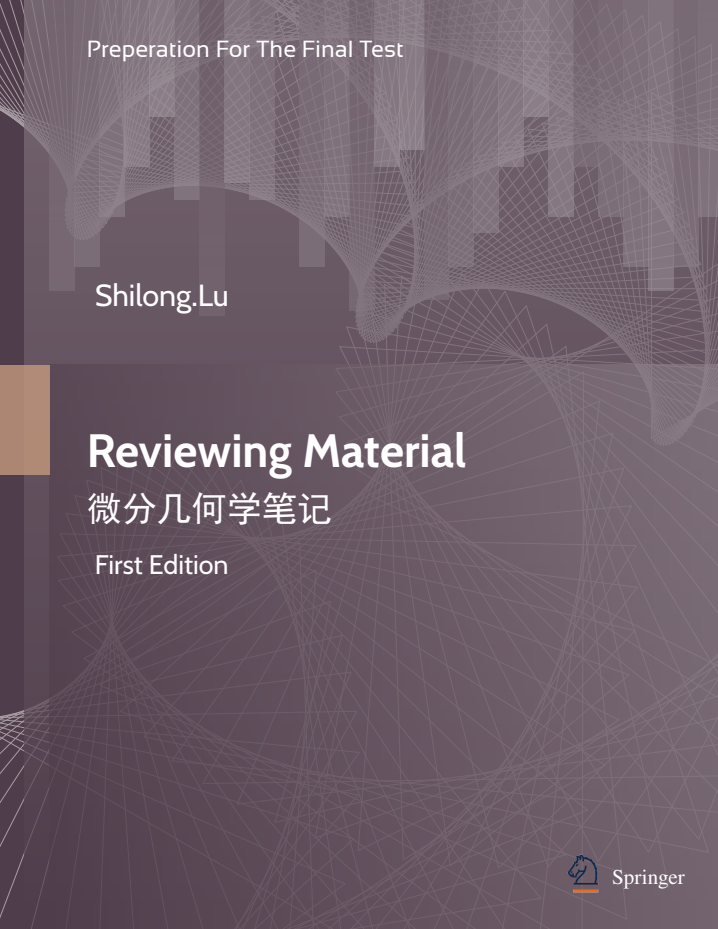
\includegraphics[width=.5\linewidth]{figures/Canonical_Springer.png}
        \caption{Springer经典封面}
        \label{Springer经典封面}
    \end{figure}
    \item Springer经典封面之二--对应宏包 \lstinline{stys/secondtitlepage}, 效果
    \begin{figure}[htbp]
        \centering
        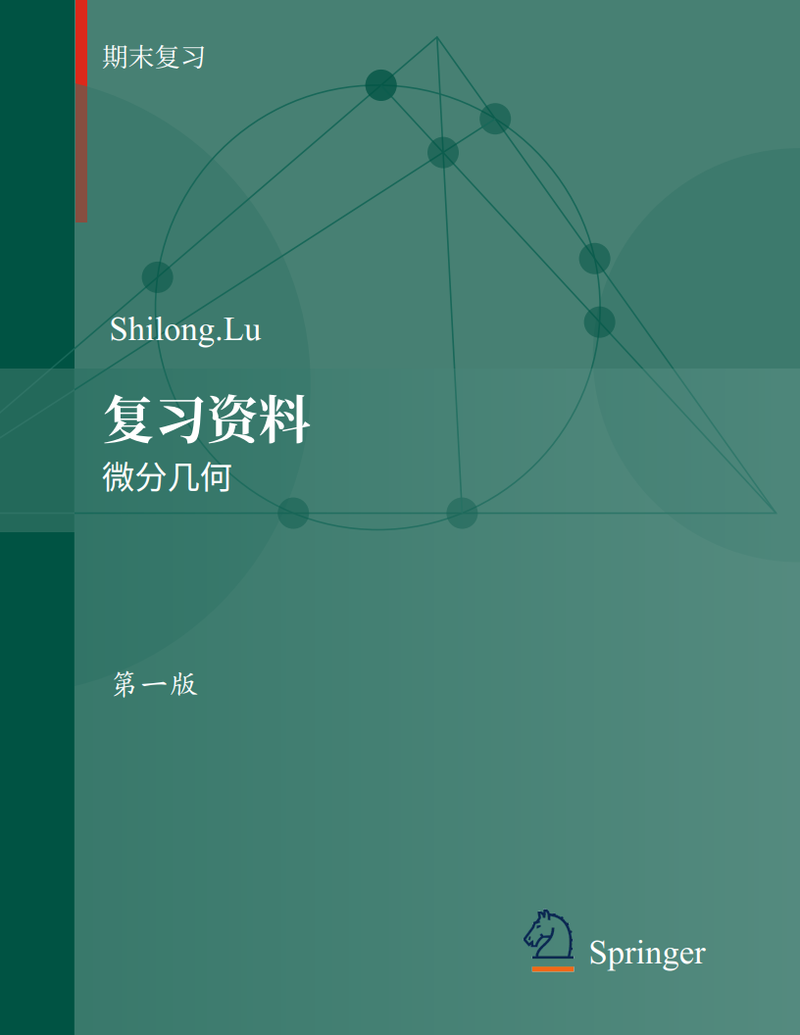
\includegraphics[width=.5\linewidth]{figures/Springer2.png}
        \caption{Springer经典封面之二}
        \label{Springer经典封面2}
    \end{figure}
    \item Springer经典封面之三--对应宏包 \lstinline{stys/imagecover},效果 
    \begin{figure}[htbp]
        \centering
        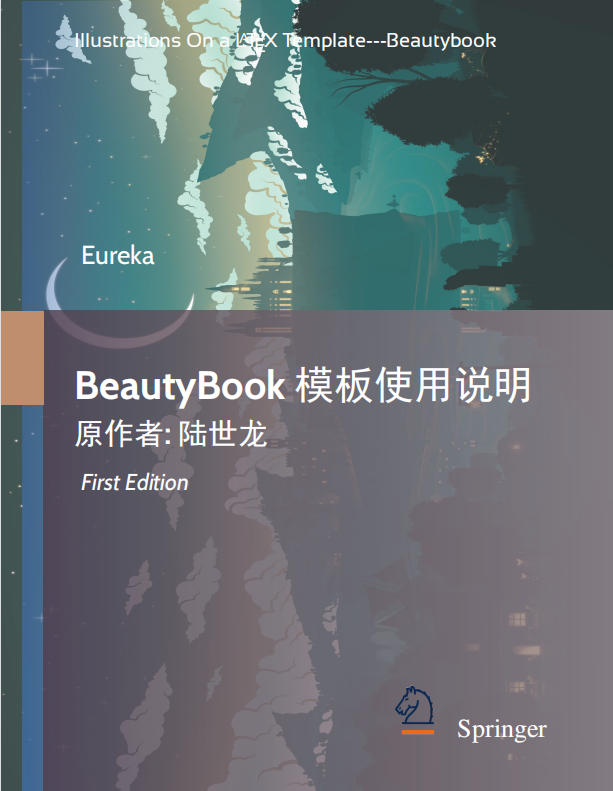
\includegraphics[width=.5\linewidth]{figures/Springer3.png}
        \caption{Springer经典封面之三}
        \label{Springer经典封面之三}
    \end{figure}
    \item 中文书籍经典封面--对应宏包\lstinline{stys/cncover},效果
    \begin{figure}[htbp]
        \centering
        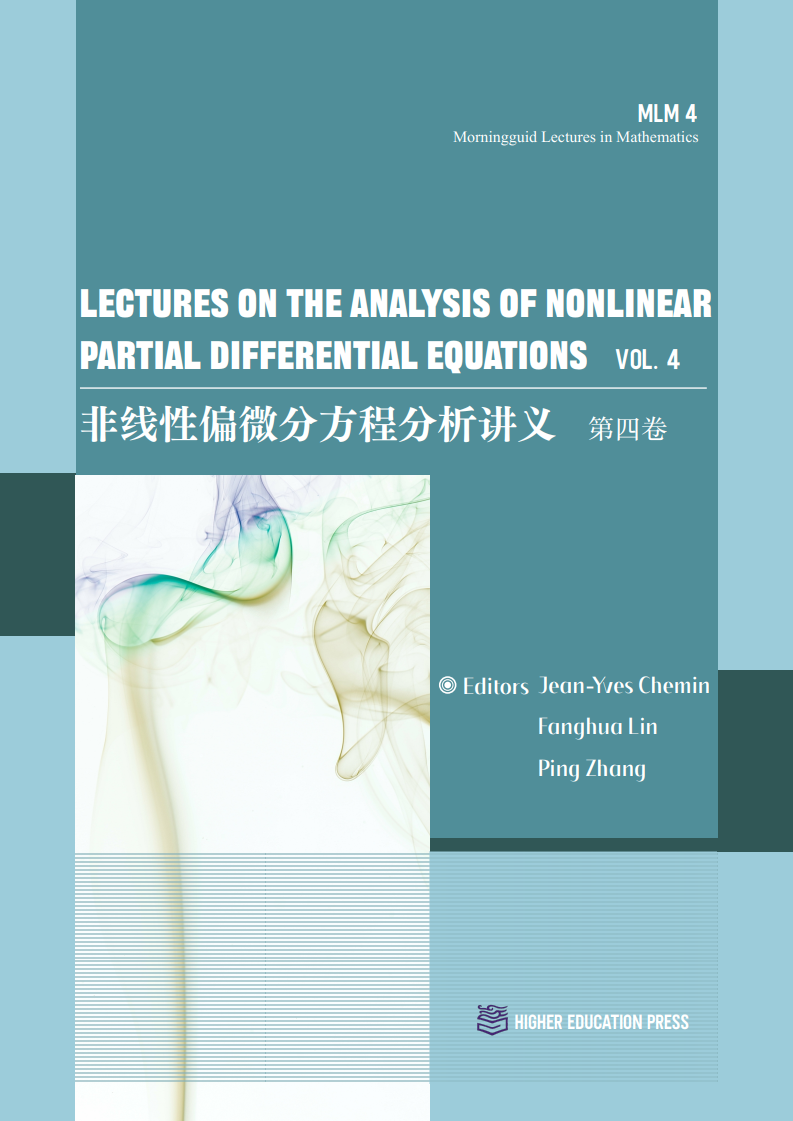
\includegraphics[width=.5\linewidth]{figures/cncover.png}
        \caption{中文书籍经典封面}
        \label{中文书籍经典封面}
    \end{figure}
    注意, 使用该封面所对应的信息不太一样, 需要在本文件基础上添加
    \begin{lstlisting}
        \englishtitle{英文标题}
        \bookseries{书籍系列}
        \chinesetitle{中文标题}
        \author{作者}
        \pressname{出版社名称}
        \presslogo{出版社logo}
        \coverimage{封面图片}
        \makecover
    \end{lstlisting}
\end{enumerate}

\begin{table}[htbp]
  \centering
  \caption{封面元素信息}
  \begin{tabular}{cccccc}
    \hline
    信息 & 命令 & 信息 & 命令 & 信息 & 命令 \\
    \hline
    标题 & \lstinline|\title| & 副标题 & \lstinline|\subtitle| & 作者 & \lstinline|\author| \\
    出版社 & \lstinline|\pressname| & 版本 & \lstinline|\edition| & 封面图 & \lstinline|\coverimage|\\
    徽标 & \lstinline|\presslogo| &&&&\\
    \hline
  \end{tabular}
\end{table}


\subsection{封面图}
封面图片可以自行去找. 

\subsection{徽标}

本文用到的 Logo 为wiki随意找的springer经典马标, 可以自己查询下载出版社logo, 为免侵权,在更换图片的时候请选择合适合法的图片进行替换。

\subsection{自定义封面}

另外,如果使用自定义的封面,比如 Adobe illustrator 或者其他软件制作的 A4 PDF 文档,请把 \lstinline{\makecover} 注释掉,然后借助 \lstinline{pdfpages} 宏包将自制封面插入即可。如果使用 \lstinline{titlepage} 环境,也是类似。

\section{章标标题}

本模板自定义了一套标题样式, 主要是 part、chapter、section 这三个标题,具体代码见cls。如果不合您的口味,可以一口气全部注释掉即可,使用上本人无权干涉, 但是鉴于审美观各异,不要说不该说的话即可!

\section{数学环境简介}

在我们这个模板中,我们定义了四种不同的定理模式,包括简单模式(默认的定理样式amsthm) 、有点自定义的thmtools、彩色强调盒子、以及本人开发的专有版权盒子,当然,由雾月老师给我定制的古风盒子您也可以是用来作为定理盒子,只需要在本文件导言区第一种定理样式里面加上\lstinline{ys style}即可.


\subsection{定理类环境的使用}
以下是使用效果展示
\subsubsection{amsthm}
\begin{lstlisting}
    
\end{lstlisting}
\begin{remark}
    这是基于amsthm的注释环境
\end{remark}
\subsubsection{thmtools}
\begin{proof}[证明的说明]
    证明环境
\end{proof}

\begin{solution}[解的说明]
    解环境
\end{solution}
\subsubsection{彩色强调盒子}
\begin{defi}[名称]\label{defi:def test}
    第一种定义环境
\end{defi}

\begin{thm}[名称]\label{thm:thm test}
    第一种定理环境
\end{thm}

\begin{cor}[名称]\label{cor:cor test}
    第一种推论环境
\end{cor}

\begin{prop}[名称]\label{prop:prop test}
    第一种命题环境
\end{prop}

\begin{exam}[名称]\label{exam:exam test}
    第一种例题环境
\end{exam}

\begin{lem}[名称]\label{lem:lem test}
    第一种引理环境
\end{lem}
\subsubsection{个人版权的盒子共两种}

\begin{definition}[][名称][def label] 
    这是个人版权的盒子定制的定理环境,这是其中定义环境示例。注意:使用方法如下

    \begin{itemize}
        \item 如果你没有名称和标签,使用方法为
    \begin{lstlisting}
        \begin{definition}
            定义环境内容
        \end{definition}
    \end{lstlisting}
        \item 如果你没有标签但有名称,使用方法为
        \begin{lstlisting}
            \begin{definition}[][名称]
                定义环境内容
            \end{definition}
        \end{lstlisting}
        \item 如果你有标签,那么无论是否有名称,使用方法为
        \begin{lstlisting}
            \begin{definition}[][有就填,没有空着][标签]
                定义环境内容
            \end{definition}
        \end{lstlisting}
        \item 如果你想更改盒子的一些设定选项,比如加框线等之类的,使用方法为
        \begin{lstlisting}
            \begin{definition}[tcolorbox选项][名称有就写,没有就连带外面括号删掉][标签 (有标签下就这样子,没有标签可以把这个标签连带外面的括号删掉)]
                定义环境内容
            \end{definition}
        \end{lstlisting}
    \end{itemize}

\end{definition}

\begin{theorem}
    用法同上,引用下上面的标签 \ref{def label}或者可以\autoref{def label}.
\end{theorem}

\begin{lemma}
    用法同上,引用下上面的标签 \ref{def label}或者可以\autoref{def label}.
\end{lemma}

\begin{corollary}
    用法同上,引用下上面的标签 \ref{def label}或者可以\autoref{def label}.
\end{corollary}

\begin{example}
    用法同上,引用下上面的标签 \ref{def label}或者可以\autoref{def label}.
\end{example}


\subsection{修改计数器}

当前定理等环境计数器按章计数,如果想修改定理类环境按节计数,可以修改计数器选项 \lstinline{ counter/.code}中的\lstinline{chapter},可用选项为 \lstinline{chapter} (默认)与 \lstinline{section}、 \lstinline{subsection}等

\subsection{自定义定理类环境}
用户可以采用四种方式定义自己的定理环境,分别为amsthm与thmtools, 这两种看宏包说明文档即可; 后面两种定理的定义方式为
如本文件导言区:
\begin{lstlisting}
    % 这是第一种
    \mynewtheorem{
        defi={\textbf{定义}}[section]{interior style={left color=ReD!8,right color=ReD!5!CyaN!50}, borderline west={1.5mm}{0mm}{ReD}},
        thm={\textbf{定理}}[section]{interior style={left color=CyaN!80!black!20,right color=CyaN!80!black!15!CyaN!50}, borderline west={1.5mm}{0mm}{CyaN!80!black}},
        lem={\textbf{引理}}[section]{interior style={left color=BluE!8,right color=BluE!5!CyaN!50}, borderline west={1.5mm}{0mm}{BluE}},
        prop={\textbf{命题}}[section]{interior style={left color=OrangE!8,right color=OrangE!5!CyaN!50}, borderline west={1.5mm}{0mm}{OrangE}},
        exam={\textbf{题}}[chapter]{interior style={left color=DarkGreen!8,right color=DarkGreen!5!CyaN!50}, borderline west={1.5mm}{0mm}{DarkGreen}},
        cor={\textbf{推论}}[chapter]{interior style={left color=violet!8,right color=violet!5!CyaN!50}, borderline west={1.5mm}{0mm}{violet}},
    }

    % 下面是第二种
    \mynewtcbtheorem{
    % 这个 theorem 是环境名
    theorem={
        counter=tcbthm, 
        the counter=\thesection.\arabic{tcbthm}, 
        name=定理, % 它保存到 \theorem@name 里
        thmcolor=purple5,
        autoref name=\bfseries 定理, 
        style={
        arc=3pt,breakable,enhanced,interior style={top color=purple5!5 ,middle color=purple5!1!nuanbai, bottom color=nuanbai},boxrule=0pt,top=8mm,
        fuzzy shadow={-0.6mm}{0.6mm}{0mm}{0.3mm}{white!50!gray},% 上
        fuzzy shadow={0.6mm}{-0.6mm}{0mm}{0.3mm}{fill=white!40!gray},%下
        opacityframe=0, opacityback=0.98,
        fontupper=\itshape, step={tcbthm},
        before pre=\smallskip, after app=\smallskip,
        overlay unbroken=\my@theorem@overlay@unbroken{\theorem@name\ \thetcbthm}{\theorem@thmcolor},
        overlay first=\my@theorem@overlay@first{\theorem@name\ \thetcbthm}{\theorem@thmcolor},
        overlay last=\my@theorem@overlay@last{\theorem@thmcolor},
        }
    },
    proposition={
        counter=tcbprop, 
        the counter=\thesection.\arabic{tcbprop}, 
        autoref name=\bfseries 命题, 
        style={
        arc=3pt,breakable,enhanced,interior style={top color=DeepPink!5 ,middle color=DeepPink!1!nuanbai, bottom color=nuanbai},boxrule=0pt,top=8mm,
        fuzzy shadow={-0.6mm}{0.6mm}{0mm}{0.3mm}{white!50!gray},% 上
        fuzzy shadow={0.6mm}{-0.6mm}{0mm}{0.3mm}{fill=white!40!gray},%下
        opacityframe=0, opacityback=0.98,
        fontupper=\itshape, step={tcbprop},
        before pre=\smallskip, after app=\smallskip,
        overlay unbroken=\my@theorem@overlay@unbroken{命题\ \thetcbprop}{DeepPink},
        overlay first=\my@theorem@overlay@first{命题\ \thetcbprop}{DeepPink},
        overlay last=\my@theorem@overlay@last{DeepPink},
        }
    },
    definition={
        counter=tcbdefi, 
        the counter=\thesection.\arabic{tcbdefi}, 
        autoref name=\bfseries 定义, 
        style={
        arc=3pt,breakable,enhanced,interior style={top color=紫棠!5 ,middle color=紫棠!1!nuanbai, bottom color=nuanbai},boxrule=0pt,top=8mm,
        fuzzy shadow={-0.6mm}{0.6mm}{0mm}{0.3mm}{white!50!gray},% 上
        fuzzy shadow={0.6mm}{-0.6mm}{0mm}{0.3mm}{fill=white!40!gray},%下
        opacityframe=0, opacityback=0.98,
        fontupper=\itshape, step={tcbdefi},
        before pre=\smallskip, after app=\smallskip,
        overlay unbroken=\my@theorem@overlay@unbroken{定义\ \thetcbdefi}{紫棠},
        overlay first=\my@theorem@overlay@first{定义\ \thetcbdefi}{紫棠},
        overlay last=\my@theorem@overlay@last{紫棠},
        }
    },
    lemma={
        counter=tcblem,
        the counter=\thesection.\arabic{tcblem},
        name=引理, 
        lemcolor=靛蓝, 
        autoref name=\bfseries 引理,
        style={
        arc=0mm,breakable,enhanced,interior style={top color=靛蓝!5 ,middle color=靛蓝!1!nuanbai, bottom color=nuanbai},arc=3pt,boxrule=0pt,top=7mm,bottom=5mm,
        fuzzy shadow={-0.6mm}{0.6mm}{0mm}{0.3mm}{white!50!gray},% 上
        fuzzy shadow={0.6mm}{-0.6mm}{0mm}{0.3mm}{fill=white!40!gray},%下
        opacityframe=0, opacityback=0.98,
        fontupper=\normalsize,step={tcblem},
        before pre=\smallskip, after app=\smallskip,
        overlay unbroken=\my@lemma@overlay@unbroken{\lemma@name\ \thetcblem}{\lemma@lemcolor},
        overlay first=\my@lemma@overlay@first{\lemma@name\ \thetcblem}{\lemma@lemcolor},
        overlay last=\my@lemma@overlay@last{\lemma@lemcolor},
        }
    },
    corollary={
        counter=tcbcor,
        the counter=\thesection.\arabic{tcbcor},
        autoref name=\bfseries 推论,
        style={
        arc=0mm,breakable,enhanced,interior style={top color=茶色!5 ,middle color=茶色!1!nuanbai, bottom color=nuanbai},arc=3pt,boxrule=0pt,top=7mm,bottom=5mm,
        fuzzy shadow={-0.6mm}{0.6mm}{0mm}{0.3mm}{white!50!gray},% 上
        fuzzy shadow={0.6mm}{-0.6mm}{0mm}{0.3mm}{fill=white!40!gray},%下
        opacityframe=0, opacityback=0.98,
        fontupper=\normalsize,step={tcbcor},
        before pre=\smallskip, after app=\smallskip,
        overlay unbroken=\my@lemma@overlay@unbroken{推论\ \thetcbcor}{茶色},
        overlay first=\my@lemma@overlay@first{推论\ \thetcbcor}{茶色},
        overlay last=\my@lemma@overlay@last{茶色},
        }
    },
    example={
        counter=tcbexam,
        the counter=\thesection.\arabic{tcbexam},
        autoref name=\bfseries 例题,
        style={
        arc=0mm,breakable,enhanced,interior style={top color=黛绿!5 ,middle color=黛绿!1!nuanbai, bottom color=nuanbai},arc=3pt,boxrule=0pt,top=7mm,bottom=5mm,
        fuzzy shadow={-0.6mm}{0.6mm}{0mm}{0.3mm}{white!50!gray},% 上
        fuzzy shadow={0.6mm}{-0.6mm}{0mm}{0.3mm}{fill=white!40!gray},%下
        opacityframe=0, opacityback=0.98,
        fontupper=\normalsize,step={tcbexam},
        before pre=\smallskip, after app=\smallskip,
        overlay unbroken=\my@lemma@overlay@unbroken{例题\ \thetcbexam}{黛绿},
        overlay first=\my@lemma@overlay@first{例题\ \thetcbexam}{黛绿},
        overlay last=\my@lemma@overlay@last{黛绿},
        }
    },
}
\end{lstlisting}
\begin{remark}
    解释一下, 其中的overlay部分更改需要看中文修改,定理名称改成你想要的,颜色也是,然后别忘了给最外面的example之类的环境名改成你的,比如axiom之类,还有就是tcbexam这个计数器名称要换成你新定义的,如tcbaxiom之类,其他就不用动了。至于说第一种定理样式看上面例子相信您能学会的。
\end{remark}

\section{列表环境}
本模板借助于 \lstinline{enumitem} 实现了可定制化,具体见enumitem宏包说明文档,这里示例如下\\[2ex]
\begin{minipage}[b]{0.49\textwidth}
  \begin{itemize}[label=$\bigodot $]
    \item first item of nesti;
    \item second item of nesti;
      \begin{itemize}
        \item first item of nestii;
        \item second item of nestii;
        \begin{itemize}
          \item first item of nestiii;
          \item second item of nestiii.
        \end{itemize}   
      \end{itemize}
  \end{itemize}
\end{minipage}
\begin{minipage}[b]{0.49\textwidth}
  \begin{enumerate}[label=\arabic*)]
    \item first item of nesti;
    \item second item of nesti;
      \begin{enumerate}
        \item first item of nestii;
        \item second item of nestii;
        \begin{enumerate}
          \item first item of nestiii;
          \item second item of nestiii.
        \end{enumerate}   
      \end{enumerate}
  \end{enumerate}
\end{minipage}

\section{参考文献}

\subsection{打印文献}

\lstinline{ref.bib} 为参考文献存放的文件,需要放在项目文件夹下。

\subsection{修改文献格式}

此外,本模板调用了 biblatex 宏包,并提供了 biber引擎编译参考文献,当然您也可以直接删除cls中的biblatex宏包(cls最后几行)来使用bibtex.

关于文献条目(bib item),你可以在谷歌学术,Mendeley,Endnote 中取,然后把它们添加到 \lstinline{ref.bib} 中。在文中引用的时候,引用它们的键值(bib key)即可。

文献样式默认为国标 GB7714-2015, 参考文献示例:\cite{2015Glypican,吴大任1979微分几何讲义,LDG} 使用了中国一个大型的 P2P 平台(人人贷)的数据来检验男性投资者和女性投资者在投资表现上是否有显著差异。

如果需要设置为数字样式,需要将biblatex宏包选项中的国标改为numerical.
\begin{lstlisting}
\usepackage[
backend=biber, % 可改为bibtex (或者直接删掉就是bibtex)
style=gb7714-2015, % 可改为 numerical
sorting=nty
]{biblatex}
\addbibresource{ref.bib}
\end{lstlisting}


\section{旁注}

本文类默认不支持旁注,如果需要旁注可以自行修改。但是需要比较高的水平,如果您确实需要,可以有偿定制 (穷学生一枚,实在缺钱也缺时间,见谅!)  一般不建议使用旁注的,因为旁注能显示的信息有限,但如果确实有需求,这边也只能有偿定制或者转到别的模板,很抱歉,这个比较小众的功能确实没法支持.


\chapter{字体选项}
字体选项独立成章的原因是,我们希望本模板的用户关心模板使用的字体,知晓自己使用的字体以及遇到字体相关的问题能更加便捷地找到答案。

本模板默认使用ctex的windows选项提供的字体, 如非必要,字体不应改动,当然,如果确实需要,可按照下面代码操作:
\begin{lstlisting}
    \setCJKmainfont[Path=fonts/,BoldFont={XX.TTF},ItalicFont={YY.TTF},SlantedFont = {ZZ.TTF} , SlantedFeatures = {FakeSlant}]{WW.TTF}
    \setCJKsansfont[Path=fonts/,BoldFont={XX.TTF},ItalicFont={XX.TTF}]{XX.TTF}
    \setCJKmonofont[Path=fonts/,BoldFont={XX.TTF},ItalicFont={XX.TTF}]{XX.TTF}
    %设置新的中文字体命令
    \newCJKfontfamily[song]\songti{XX.TTF}[Path=fonts/] %宋体
    %设置新的英文字体命令
    \newfontfamily\largetitlestyle[Path=fonts/]{XX.TTF}
\end{lstlisting}

\section{数学字体选项}
本模板使用的是mtpro2字体,需要用户自行安装,安装教程见\href{https://www.latexstudio.net/archives/51742.html}{mtpro2字体安装教程}。当然也可以删除本文件导言区的mtpro2字体换回默认数学字体,诸君随意。

\chapter{Beautybook 写作示例}
见文件夹中附带的我的笔记.在此不再赘述.

\chapter{常见问题解决方法}
随后更新

\chapter{版本更新历史}

\setcounter{part}{9998}
\setcounter{chapter}{9998}
\setcounter{section}{9998}
\chapter{超长标题测试超长标题测试超长标题测试超长标题测试超长标题测试超长标题测试超长标题测试超长标题测试超长标题测试}
\section{超长标题测试超长标题测试超长标题测试超长标题测试超长标题测试超长标题测试超长标题测试超长标题测试超长标题测试}
这里演示了为何章与节是这样子设计的? 主要是为了信息不冲突,兼容性更好,可以像原本默认的标题一样,任意使用都不会产生问题.
\clearpage
\section{{2}}
\backmatter
\normalem
\printbibliography[
heading=bibintoc,
title={参考文献}
]
\printindex
\thispagestyle{empty}
\bottomimage{figures/M31OiiiArc_Strottner_5000.jpg}
\summary{封底信息.}
\makebottomcover
\end{document} 